\documentclass{article}
\usepackage[utf8]{inputenc}
\usepackage[margin = 0.8in]{geometry}
\usepackage{graphicx}
\usepackage{amsmath, amssymb}
\usepackage{subcaption}
\usepackage{multirow}
\usepackage{mathtools}
\usepackage{float}


\title{RBE502 - Homework Set 9}
\author{Keith Chester}
\date{Due date: November 3 2021}

\begin{document}
\maketitle

\section*{Introduction}
In this assignment, we are charged with exploring various path planning algorithms - specifcally depth-first-search (DFS), breadth-first-search (BFS), and Dijkstra's search. We also explore A* and greedy search algorithms for comparison.

In this project, we are looking at a discrete space of a square grid. The grid consists of individual cells that are represented as occupied by an obstacle (a black square), as empty (a white square), the robot's starting position (a red square), and the goal (a green square). In our provided examples, an additional light blue square is used to show areas that were considered during path planning, but not utilized, and a dark blue square for the final generated path. For movement, we only consider orthogonal movement, no diagonals.

\section*{Examples}
Here we see a an example map of 128x128 grid cells. In this example, we fill the map with obstacles until we hit a desired coverage percentage - in this case, $ 35\% $ coverage. We see the total considered cells and final path from the robot's starting position to its goal.

\begin{figure}[H]
    \centering
    \begin{subfigure}{0.325\textwidth}
        \centering
        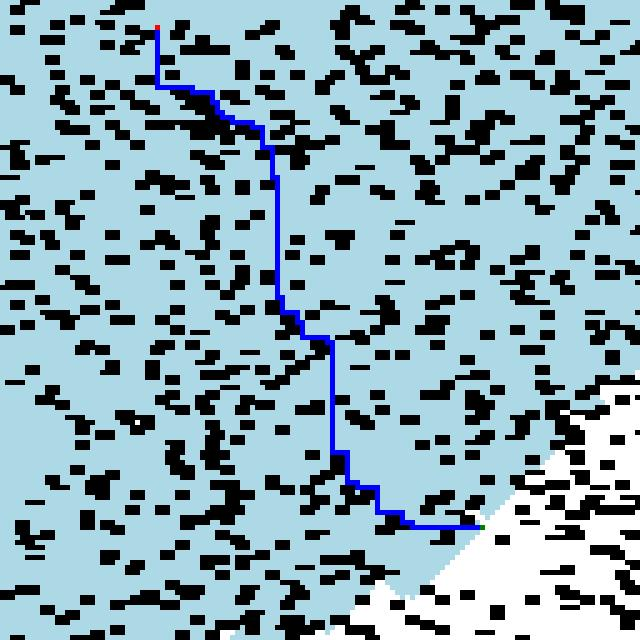
\includegraphics[width = \textwidth]{images/bfs.jpg}
        \caption{Breadth first search (BFS)}
    \end{subfigure}
    \begin{subfigure}{0.325\textwidth}
        \centering
        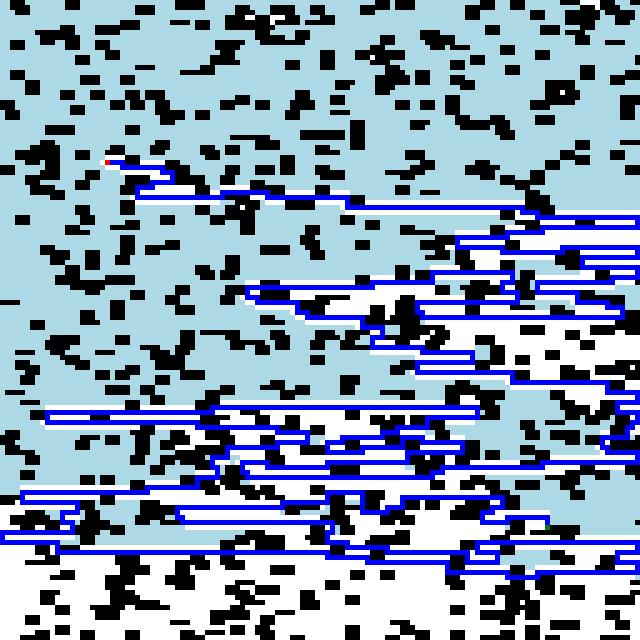
\includegraphics[width = \textwidth]{images/dfs.jpg}
        \caption{Depth first search (DFS)}
    \end{subfigure}
    \begin{subfigure}{0.325\textwidth}
        \centering
        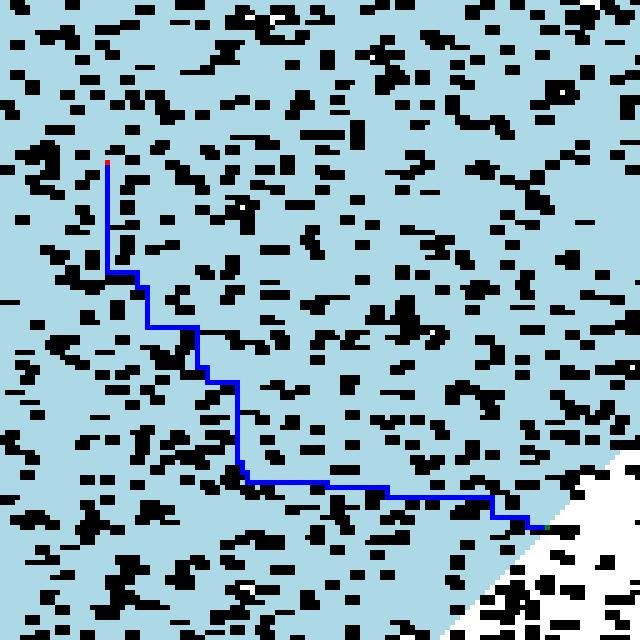
\includegraphics[width = \textwidth]{images/dijkstras.jpg}
        \caption{Dijkstras}
    \end{subfigure}
    \begin{subfigure}{0.325\textwidth}
        \centering
        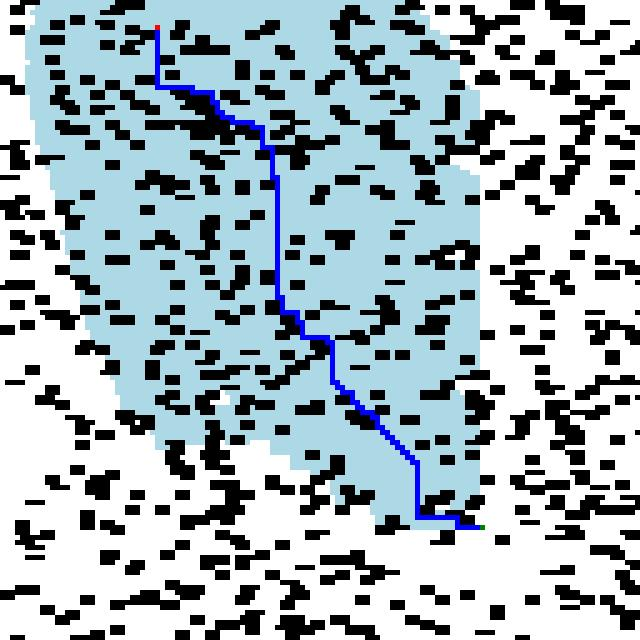
\includegraphics[width = \textwidth]{images/astar.jpg}
        \caption{A*}
    \end{subfigure}
    \begin{subfigure}{0.325\textwidth}
        \centering
        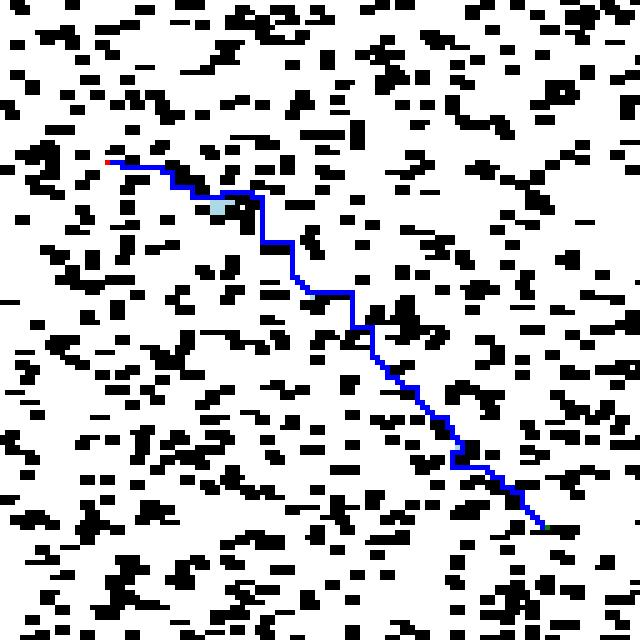
\includegraphics[width = \textwidth]{images/greedy.jpg}
        \caption{Greedy}
    \end{subfigure}
    \caption{Example maps with solved paths for each algorithm}
    \label{fig:example-maps}
\end{figure}

TODO - DISCUSSION OF WHAT SEE ABOVE

\section*{Performance}

We took each algorithm and plot total iterations taken to find a solution and the resulting path length, as well as all algorithms overlayed. We explored each algorithm from $0\%$ obsacle coverage to $75\%$ coverage with increments of $5\%$. For each algorithm and percentage combination, we randomly generate 500 solvable maps and perform the solution. If a generated map was not solvable (no path existed), we would ignore that attempt for our total of 500.

The individual performance of each algorithm is shown below:

\begin{figure}[H]
    \centering
    \begin{subfigure}{0.325\textwidth}
        \centering
        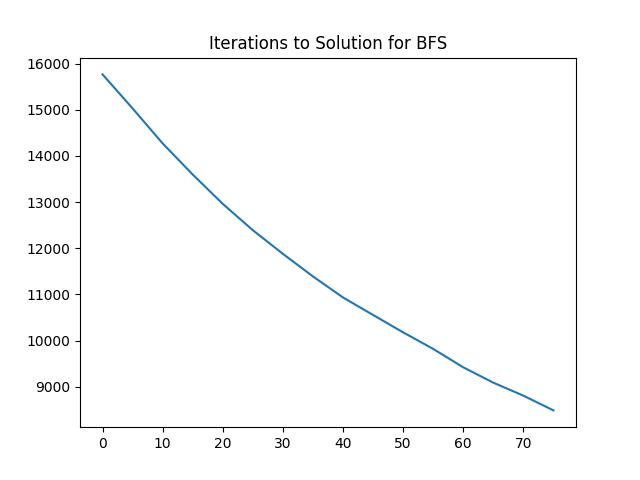
\includegraphics[width = \textwidth]{plots/BFS_iterations.jpg}
        \caption{Breadth first search (BFS)}
    \end{subfigure}
    \begin{subfigure}{0.325\textwidth}
        \centering
        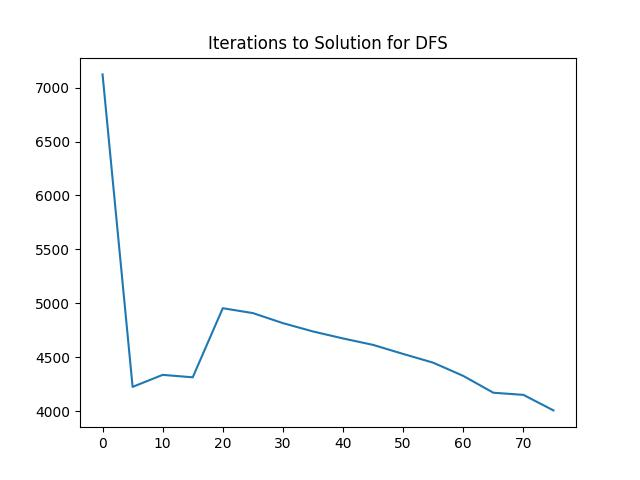
\includegraphics[width = \textwidth]{plots/DFS_iterations.jpg}
        \caption{Depth first search (DFS)}
    \end{subfigure}
    \begin{subfigure}{0.325\textwidth}
        \centering
        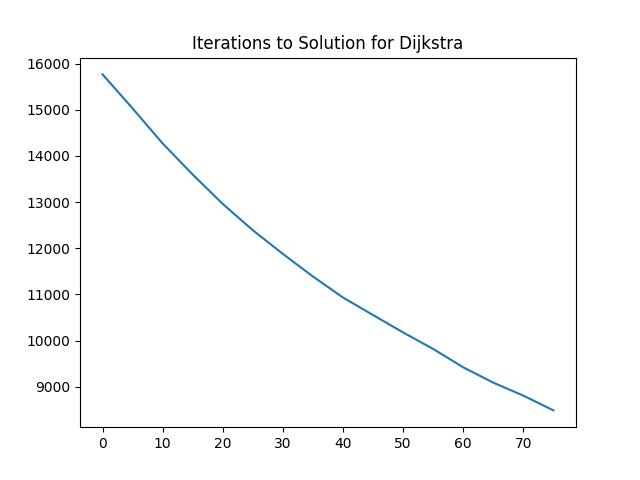
\includegraphics[width = \textwidth]{plots/Dijkstra_iterations.jpg}
        \caption{Dijkstras}
    \end{subfigure}
    \begin{subfigure}{0.325\textwidth}
        \centering
        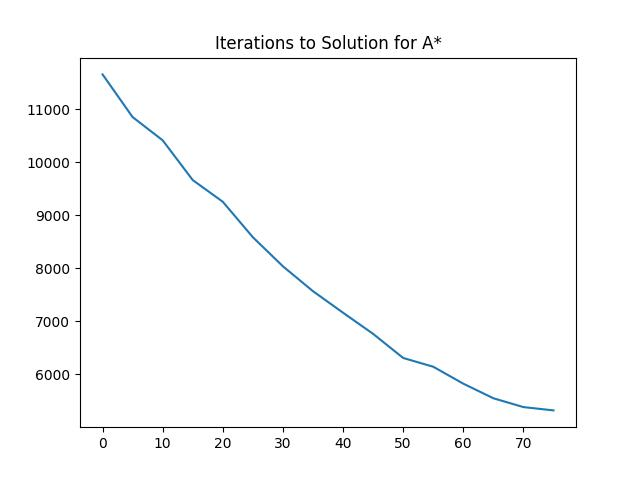
\includegraphics[width = \textwidth]{plots/A*_iterations.jpg}
        \caption{A*}
    \end{subfigure}
    \begin{subfigure}{0.325\textwidth}
        \centering
        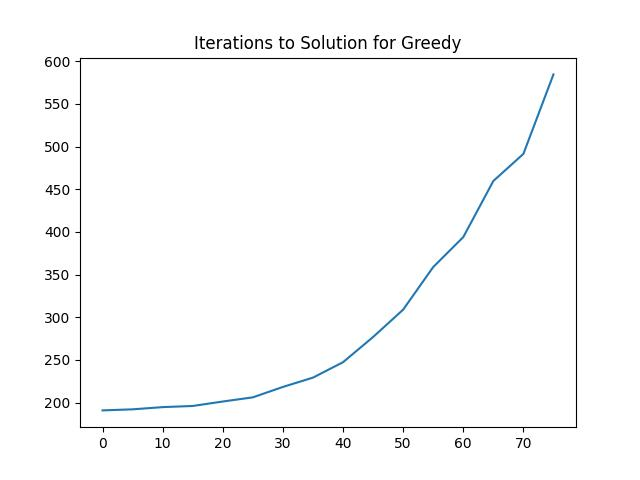
\includegraphics[width = \textwidth]{plots/Greedy_iterations.jpg}
        \caption{Greedy}
    \end{subfigure}
    \caption{Iterations per planner algorithm}
    \label{fig:iterations-per-planner}
\end{figure}

\begin{figure}[H]
    \centering
    \begin{subfigure}{0.325\textwidth}
        \centering
        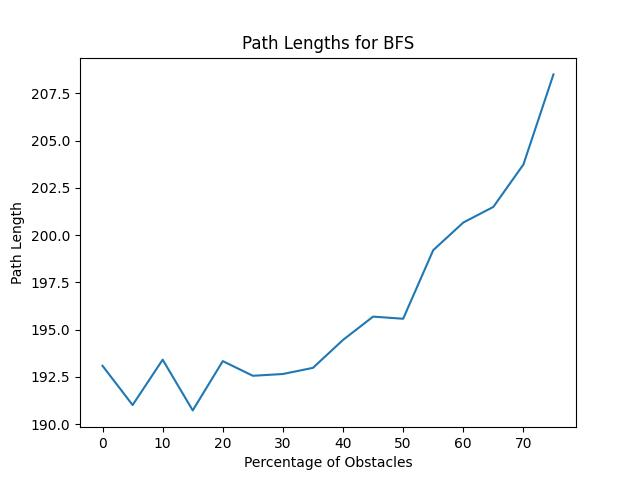
\includegraphics[width = \textwidth]{plots/BFS_paths.jpg}
        \caption{Breadth first search (BFS)}
    \end{subfigure}
    \begin{subfigure}{0.325\textwidth}
        \centering
        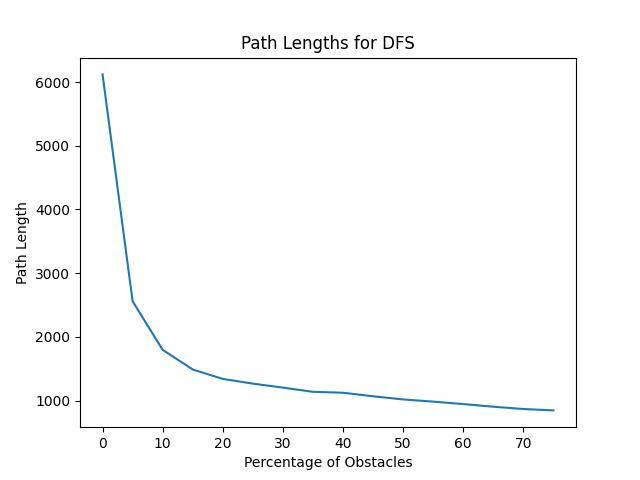
\includegraphics[width = \textwidth]{plots/DFS_paths.jpg}
        \caption{Depth first search (DFS)}
    \end{subfigure}
    \begin{subfigure}{0.325\textwidth}
        \centering
        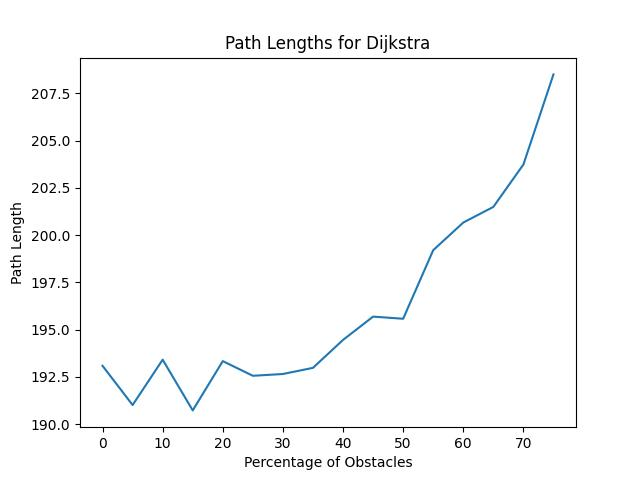
\includegraphics[width = \textwidth]{plots/Dijkstra_paths.jpg}
        \caption{Dijkstras}
    \end{subfigure}
    \begin{subfigure}{0.325\textwidth}
        \centering
        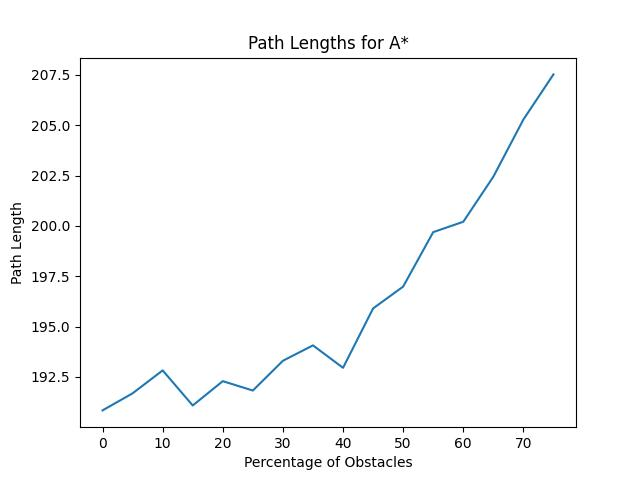
\includegraphics[width = \textwidth]{plots/A*_paths.jpg}
        \caption{A*}
    \end{subfigure}
    \begin{subfigure}{0.325\textwidth}
        \centering
        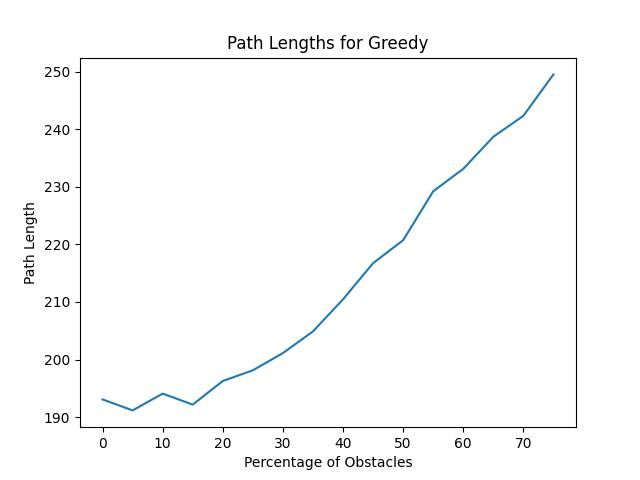
\includegraphics[width = \textwidth]{plots/Greedy_paths.jpg}
        \caption{Greedy}
    \end{subfigure}
    \caption{Path length averag per each planner algorithm}
    \label{fig:paths-per-planner}
\end{figure}

Finally, we overlay the data for planner for comparison:

\begin{figure}[H]
    \centering
    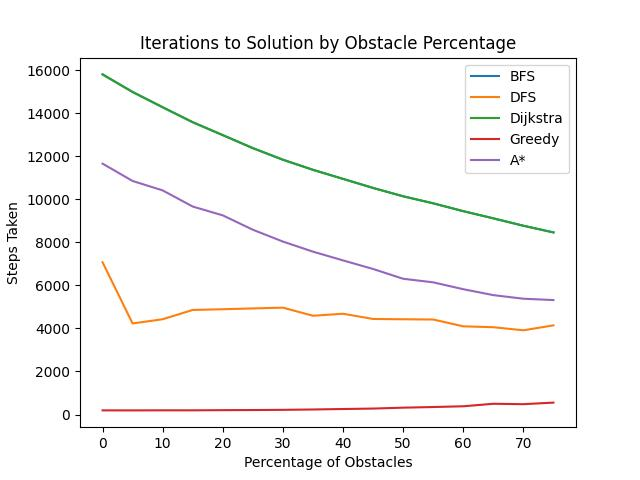
\includegraphics[width = 0.75\textwidth]{plots/steps_taken.jpg}
    \caption{Iterations for each planner algorithm overlayed}
    \label{fig:iterations-all}
\end{figure}

\begin{figure}[H]
    \centering
    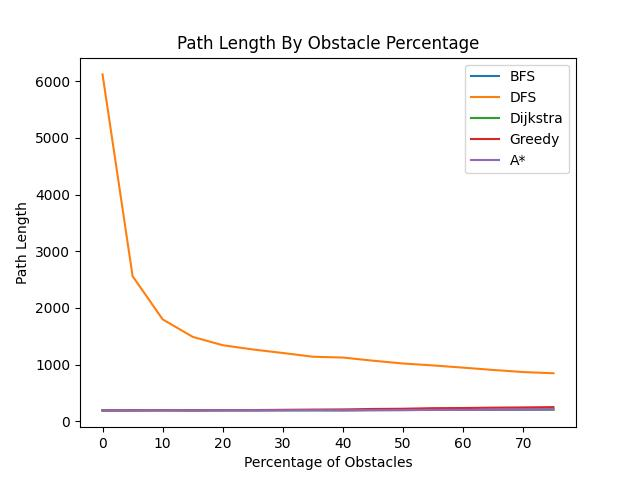
\includegraphics[width = 0.75\textwidth]{plots/path_length.jpg}
    \caption{Iterations per planner algorithm}
    \label{fig:paths-all}
\end{figure}

...and since DFS creates such inefficient routes, we look at that last chart again with DFS removed:

\begin{figure}[H]
    \centering
    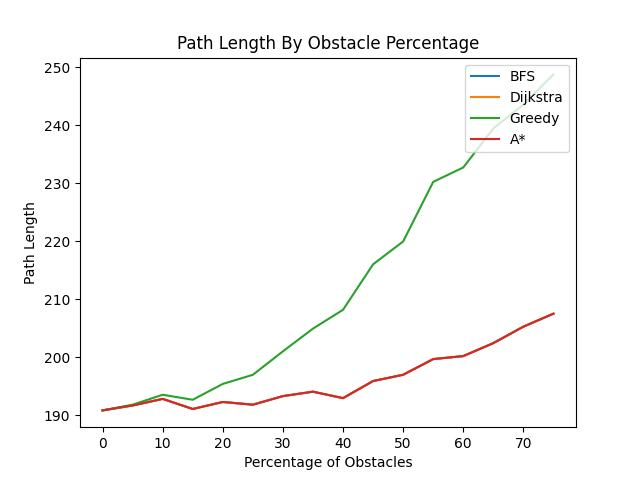
\includegraphics[width = 0.75\textwidth]{plots/path_length_sans_dfs.jpg}
    \caption{Iterations per planner algorithm, sans DFS}
    \label{fig:paths-sans-dfs}
\end{figure}

In these figures we see on our overlayed algorithms several algorithms overlap, resulting in some algorithms appearing as if they are missing. This is explained in our below section.

\section*{Results}

TODO - what we noticd, DFS vs BFS difference, greedy performance, etc


\end{document}